% \chapter{\tool ---补丁定位方法}

\chapter{开源软件漏洞的补丁识别方法}

本章将详细阐述\tool ---一种基于多源知识的开源软件漏洞的补丁识别方法的设计。

\section{方法概述}
\begin{figure*}[h]
    \centering
    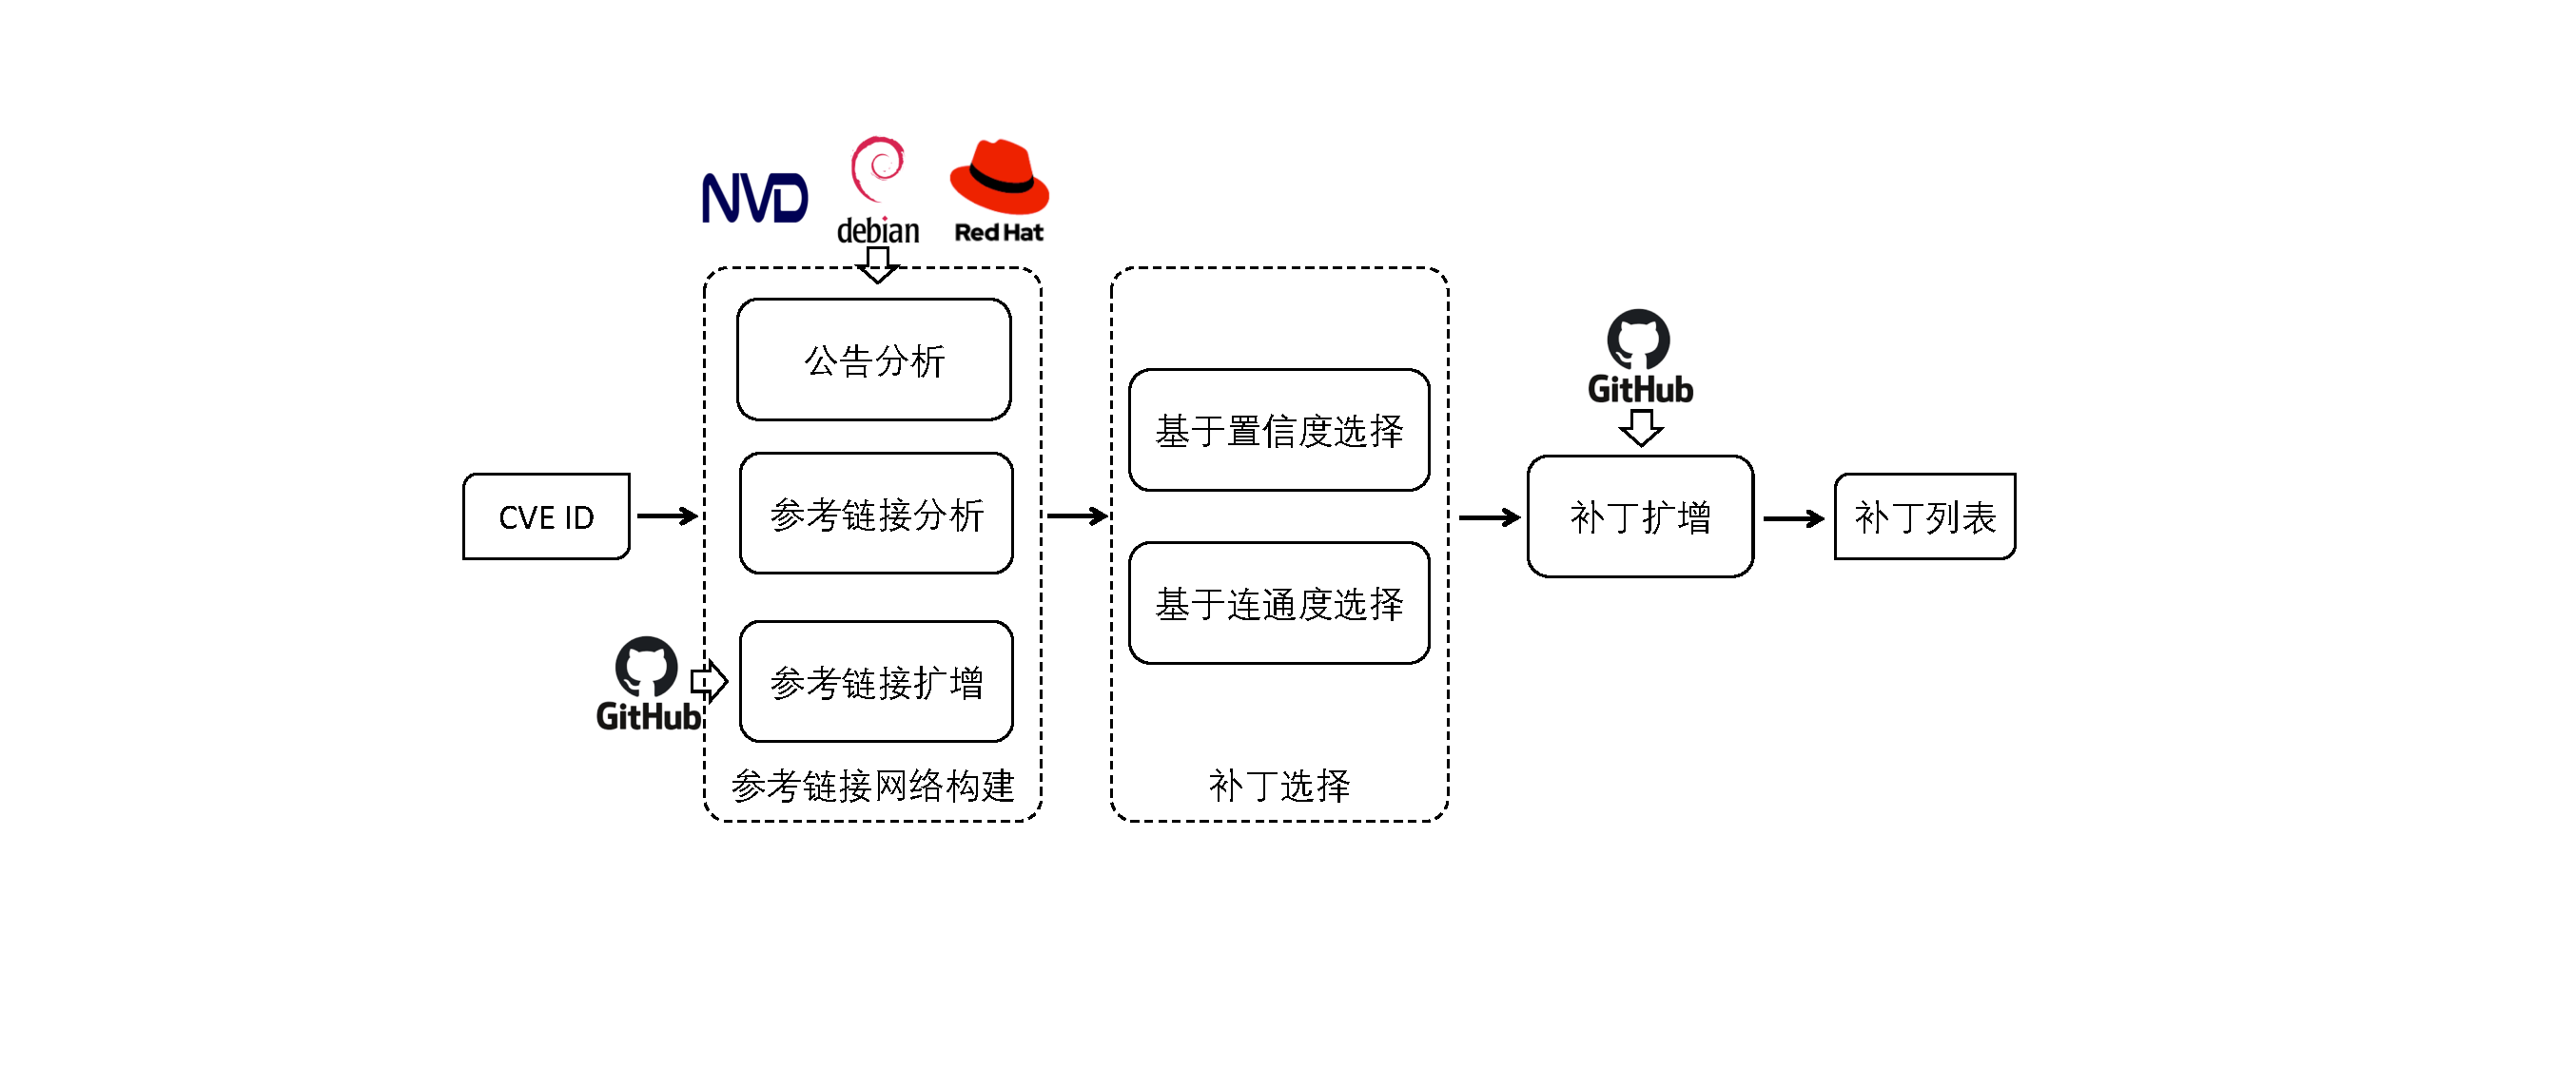
\includegraphics[scale=0.40]{fig/overview.pdf}
    %\vspace{-10pt}
    \caption{\tool 方法概览}\label{fig:overview}
\end{figure*}

基于上一章经验研究的发现,本章设计了一种名为\tool 的自动化方法来查找开源软件漏洞的补丁。该方法的核心思想是:漏洞的补丁(即Commit URL)会在与该漏洞相关的各种来源的漏洞公告、分析报告、讨论和解决的过程中被频繁提及和引用;因此,本文首先设计了一种基于多知识源的漏洞参考链接网络,再从该网络中选出具有最高置信度和连通度的补丁节点作为结果返回。

图\ref{fig:overview}为\tool 的方法概览,其中,\tool 以漏洞的CVE ID作为输入,主要经过三个步骤,最终返回其补丁。步骤一:构建多源信息网络,该步骤的目的是将该CVE在被报告、讨论和解决阶段的参考链接信息进行建模。\tool 从多个\tocheck{漏洞知识源}(即NVD、Debian\footnote{https://security-tracker.debian.org/tracker/}、Red Hat\footnote{https://bugzilla.redhat.com/}和GitHub)中提取与该CVE相关的参考链接信息并构建一个信息网络,这里将NVD视为主知识源,将Debian、Red Hat和GitHub视为次知识源,次级知识源列表可以灵活扩展。步骤二:精选补丁节点,\tool 从构建的参考链接网络中选择中具有高连通性和高置信度的补丁节点作为该CVE的补丁。步骤三:候选补丁扩增, 经验研究中发现CVE与其补丁之间存在一对多的映射关系,对此,基于步骤二中选定的补丁,\tool 通过搜索同一代码库所有分支中的相关提交(Commit)来扩展候选补丁集。最终,\tool 将该CVE的候选补丁集返回给用户,用户可基于\tool 提供的信息选定确认正确的补丁。%在本章的其他小节中,将详细阐述每个步骤。
三个步骤的具体设计和实现将在下文中详细阐述。

% \begin{itemize}[leftmargin=*]
% \item 首先,\tool 从多个\tocheck{信息源}(即NVD、Debian\cite{debian}、RedHat\cite{redhat}和GitHub)为输入的CVE构建一个相关参考链接的网络。该步骤的目的是将CVE在报告、讨论和解决阶段的参考链接信息进行建模。这里将NVD视为主信息来源,将Debian、RedHat和GitHub视为次级信息来源,该级信息源可以进一步扩展。
% \item 其次,\tool 从构建的参考链接网络中,选择中具有高连通性和高置信度的补丁节点(即commit)作为该CVE的补丁。
% \item 最后,\tool 通过搜索同一存储库中其他分支上的相关提交来扩展补丁集。该步骤目的是在CVE及其补丁之间建立潜在的一对多映射关系。
% \end{itemize}

\section{参考链接网络构建}
% \section{步骤一:构建多源参考链接网络}
\tool 的步骤一为构建漏洞参考链接网络,一共包括三个子步骤。前两个子步骤为漏洞公告节点分析和引用节点分析,通过分析来自NVD、Debian和Red Hat三个知识源的漏洞公告及其中的引用信息,构建初始参考链接网络;第三个子步骤为\tocheck{知识源扩增},从GitHub平台搜索相关的代码提交,作为补丁节点扩充入信息网络。

\subsection{公告分析} \label{sec:advisory analysis}
% 首先,\tool 初始化信息网络,将输入的CVE ID设置为根节点,获取三个漏洞知识源(即NVD、Debian和Red Hat)中该漏洞的公告,并将三个公告节点添加为根节点的子节点。这些公告节点便于后期追溯选定的补丁的信息来源。
首先,\tool 初始化信息网络,将输入的CVE ID设置为根节点,并将三个漏洞知识源(即NVD、Debian和Red Hat)中该漏洞的公告作为公告节点添加为根节点的子节点。这些公告节点便于后期追溯选定的补丁的信息来源。

\begin{figure}[h]
    \centering
    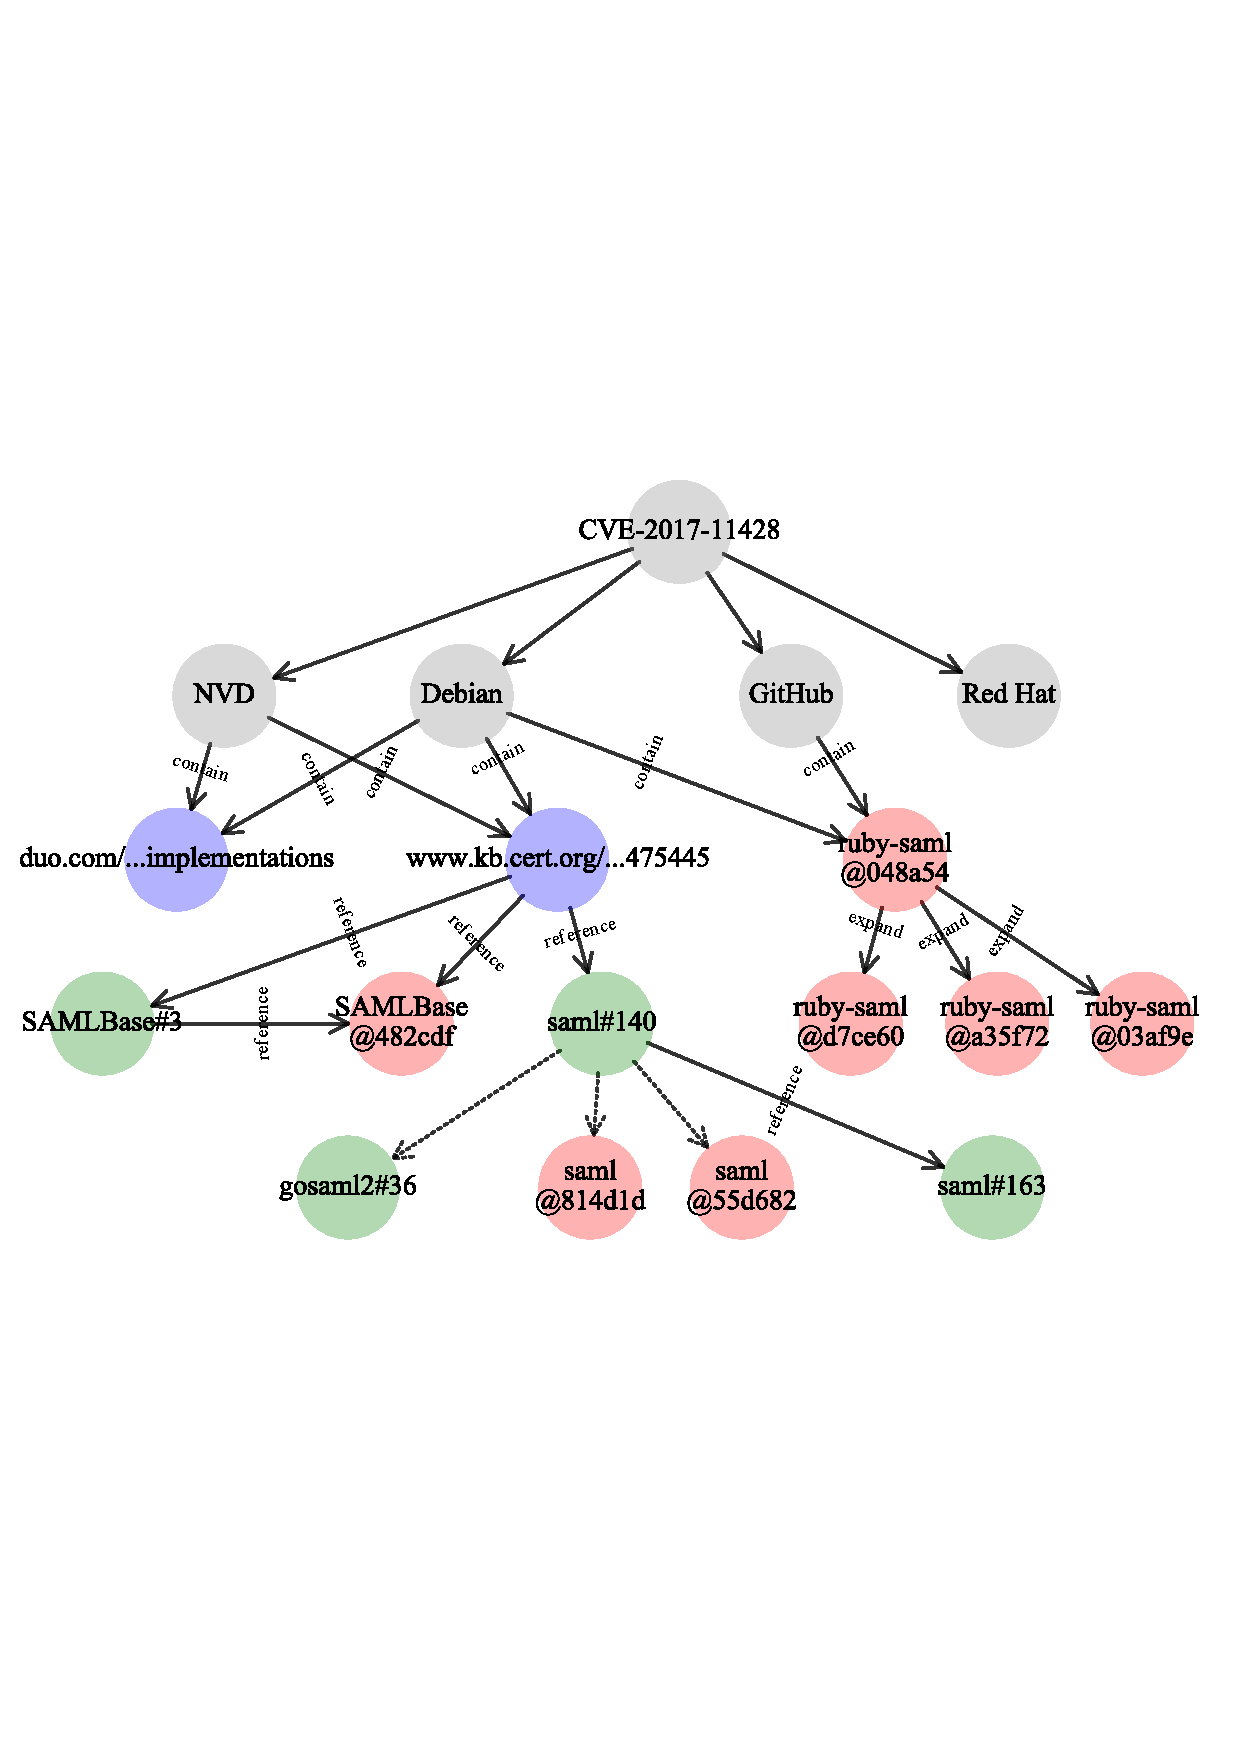
\includegraphics[scale=0.68]{fig/network-example.pdf}
    %\vspace{-10pt}
    \caption{样例CVE-2017-11428的多源参考链接网络}\label{fig:example}
\end{figure}

% \begin{table*}
%     \centering
%     \footnotesize
%     \caption{Temp  ref for Fig \ref{fig:An Example of toolname}}
%     \vspace{-10pt}
%     \begin{tabular}{|l|l|}
%     \noalign{\hrule height 1pt}
%     Identifier & URL\\\noalign{\hrule height 1pt}
%     N & https://nvd.nist.gov/vuln/detail/CVE-2017-11428\\
%     D & https://security-tracker.debian.org/tracker/CVE-2017-11428\\
%     R & https://bugzilla.redhat.com/show\_bug.cgi?id=CVE-2017-11428\\
%     ations & https://duo.com/blog/duo-finds-saml-vulnerabilities-affecting-multiple-implementations\\
%     475445 & https://www.kb.cert.org/vuls/id/475445\\
%     048a54 & https://nvd.nist.gov/vuln/detail/CVE-2017-11428\\
%     3 & https://github.com/Wizkunde/SAMLBase/issues/3\\
%     140 & https://github.com/crewjam/saml/pull/140\\
%     482cdf & https://github.com/onelogin/ruby-saml/commit/048a544730930f86e46804387a6b6fad50d8176f\\
%     d7ce60 & https://github.com/onelogin/ruby-saml/commit/d7ce607d9f9d996e1046dde09b675c3cf0c01280\\
%     a35f72 & https://github.com/onelogin/ruby-saml/commit/a35f7251b86aa3b7caf4a64d8a3451f925e8855c\\
%     03af9e & https://github.com/onelogin/ruby-saml/commit/03af9e33d2d87f4ac9a644c5b0981ded4dca0bb8\\
%     55d682 & https://github.com/crewjam/saml/commit/55d682de6bbefc17e979db16292f115467916919\\
%     814d1d & https://github.com/crewjam/saml/commit/814d1d9c18457deeda08cbda2d38f79bedccfa62\\
%     163 & https://github.com/crewjam/saml/issues/163\\
%     141 & https://github.com/crewjam/saml/pull/141\\
%     \noalign{\hrule height 1pt}
%     \end{tabular}
% \end{table*}

\begin{exmp}
图\ref{fig:example}为样例CVE-2017-11428的多源参考链接网络。 其中,最顶层为根节点(即CVE ID),第二层为公告节点(即“知识源”)。
\end{exmp}

然后,\tool 通过网络请求分别获取NVD、Debian和Red Hat平台中该CVE的漏洞公告。NVD平台中,漏洞公告以JSON形式按年份存储于结构化数据\footnote{https://nvd.nist.gov/vuln/data-feeds}中,\tool 通过下载并解析相应的JSON文件即可获得NVD中该CVE的公告信息。Debian平台中,漏洞公告也以结构化数据的形式存储在仓库\footnote{https://salsa.debian.org/security-tracker-team/security-tracker/-/tree/master/data/CVE}中,\tool 可直接从中解析得Debian提供的该CVE公告信息。Red Hat平台提供了WebService API\footnote{https://bugzilla.redhat.com/docs/en/html/api/index.html}服务,\tool 可以直接使用该服务来检索Red Hat平台的漏洞公告。值得注意的是,分析发现:Debian会跟踪NVD上的所有漏洞,而Red Hat并非跟踪所有漏洞。

\tool 从每个知识源的漏洞公告中提取引用的链接信息(即URL),并将它们添加为相应公告节点的子节点。对于NVD公告,\tool 从“references”字段中直接获取取出相关URL;类似地,对于Debian公告,\tool 直接从“Notes”字段中提取出相关URL;而对于Red Hat公告,\tool 使用正则表达式从评论区(“comments”字段)中提取出相关URL,这是因为开发人员常常会在评论区讨论和记录漏洞的解决过程并列出对补丁,但NVD和Debian平台尚未开发评论区模块。

\begin{exmp}
如图\ref{fig:example}中的第三层所示,对于CVE-2017-11428,NVD公告中包含了两个参考链接。链接一\footnote{https://duo.com/blog/duo-finds-saml-vulnerabilities-affecting-multiple-implementations}是对描述此漏洞细节的博客的引用,链接二\footnote{https://www.kb.cert.org/vuls/id/475445}是对该漏洞的第三方公告的引用。同时,这两个参考链接也包含在Debian公告中,不过Debian公告还包含修复此漏洞的GitHub提交链接ruby-saml@048a54\footnote{https://github.com/onelogin/ruby-saml/commit/048a544730930f86e46804387a6b6fad50d8176f}。此外,Red Hat平台并未收录该CVE,所以也无参考链接信息。
\end{exmp}

\tool 基于参考链接信息的内容,将引用节点分为三种类型:补丁节点(Patch Node)、\tocheck{问题节点}(Issue Node)和\tocheck{混合节点}(Hybrid Node)。这里区分出补丁节点,是因为该方法的根本目的就是在多个知识源中找到所引用的补丁。识别补丁节点的方法为:如果URL链接中包含“git”字段且可通过正则表达式匹配到Commit-ID,则该链接为Git Commit形式的补丁节点;如果URL链接中包含“svn”字段且可通过正则表达式匹配到Commit-ID,则该链接为SVN Commit形式的补丁节点。区分出问题节点是因为开发人员常常会在问题追踪系统(Issue Tracker)中讨论该issue的解决方案并引用补丁链接信息,所以,问题报告(Issue Report)是一种较为特殊且重要的引用信息;此外,问题追踪系统(Issue Tracker)中CVE相关的问题报告会有一个标识符(Issue-ID),开发人员常常会将Issue-ID写入代码提交信息(即Commit Message)中。识别问题节点的方法为:如果URL链接中包含“/github.com/”和“/issues/”,则该链接为GitHub issue形式的问题节点;如果URL链接中包含“/github.com/”和“/pull/”,则该链接为GitHub pull request形式的问题节点;如果URL链接中包含“bugzilla”、“jira”、“issues”、“bugs”、“tickets”和“tracker”中的某一个字段且可通过正则表达式匹配到issue-id,\tocheck{则该链接为通常issue tracker形式的问题节点}。对于所有未识别为补丁或问题节点的参考链接信息将被视为混合节点,它们多为博客、第三方漏洞公告等。

%受经验研究中补丁类型分析结果启发(Sec.\ref{sec:type}),

\begin{exmp}
如图\ref{fig:example}中的第三层所示,NVD和Debian公告中包含的两个参考链接被标识为混合节点(即图中的两个紫色节点),仅有一个在Debian公告中的参考链接被识别为补丁节点(即图中的红色节点)。
\end{exmp}

\subsection{参考链接分析}
对于在先前的子步骤中已添加入图的每个引用节点,\tool 将通过以下两种节点分析方式,以分层的方式继续扩建参考链接网络。%\tool 将通过“引用分析”和“信息增强”两个步骤以分层方式继续构建参考链接网络。

\textbf{方式一:}如果该引用节点的类型为补丁节点,\tool 会通过网络请求该次代码提交(Commit)的内容并分析该代码提交是否只涉及了测试代码或非源代码文件的修改。如果是的话,则表明该代码提交一定不是用于修复漏洞的补丁,\tool 会从网络中删除该节点。对于测试代码的判定,\tool 通过检查修改的文件路径中是否含有“test”字段来判断,如果文件路径含有“test”字段则判定为测试文件。对于非源代码文件的判定,\tool 通过检查修改文件的后缀来识别该文件是否为代码文件,如果文件的后缀非常见代码文件类型,即不在列表\footnote{常见代码文件后缀列表:['java', 'py', 'c', 'cc', 'cpp', 'cxx', 'c++', 'js', 'go', 'rb', 'cs', 'as', 'php', 'pl', 'coffee', 'h', 'm', 'ts', 'kt', 'mjs', 'twig', 'htaccess', 'tpl', 'pt', 'scala', 's', 'erb', 'swf', 'asm', 'groovy', 'jsp', 'sh', 'hpp', 'phps', 'script', 'wscript', 'ldif', 'Tokens', 'nsi', 'tcl', 'idl', 'pyx', 'ps1', 'toml', 'inl', 'x', 'S', 'hbs']}中则判定为非源代码文件。

\textbf{方式二:}如果该引用节点的类型为问题节点或混合节点,\tool 会通过网络请求该URL的页面信息(即HTML文本),并解析出该网页中的URL引用信息,将其作为子节点扩入引用网络。首先,对于网页中URL引用信息的提取,\tool 使用正则表达式提取纯文本中的URL引用信息,同时使用HTML解析器提取超链接(即\textbf{<a>}标签)中的URL引用信息。
然后,使用前一子步骤(\ref{sec:advisory analysis})中相同的方式识别提取的URL类型,以识别出补丁和问题引用,并将这些引用添加为当前节点的子节点。值得注意的是,在该步骤及以后流程中网络将不再加入混合节点。这是因为混合节点极易引入噪声,随着构建的越深噪声也就就越多,所以,除了直接被NVD、Debian和Red Hat公告节点引用的混合节点,其他节点分析中将不再考虑混合节点。此外,考虑到GitHub Issue中通常还包含来自其他软件仓库的问题或提交的引用,这也会给网络带来过多的噪音且使网络空间爆炸。因此,在该步骤中,如果被分析的引用节点为GitHub Issue,则仅仅将其引用的同一代码仓库中的代码提交或问题引用节点添加到网络中。

对于所有新增的节点,\tool 将一直重复以上两种节点分析的方式迭代扩增网络,直到没有任何新增的节点或者网络深度达到设定的阈值(网络深度默认为\tocheck{5}层)。

\begin{exmp}
在第一次迭代中,因为ruby-saml@048a54并非仅涉及测试代码或非源代码文件的更改,所以\tool 将补丁节点ruby-saml@048a54保留在图\ref{fig:example}中第三层;此外,\tool 标识还出第三层中的两个混合节点,其中一个混合节点未引用任何问题或提交信息,另一个混合节点了引用了两个问题链接SAMLBase\#3和saml\#140以及一个代码提交链接SAMLBase@482cdf。 

在第二次迭代中,\tool 发现节点SAMLBase\#3引用了SAMLBase@482cdf,而节点saml\#140引用了两个问题链接gosaml2\#36和saml\#163以及两个代码提交链接saml@814d1d和saml@55d682。考虑到gosaml2\#36与saml\#140并不属于同个代码仓库,saml@814d1d和saml@55d682也仅涉及测试代码的更改,\tool 便不将它们添加到网络中。为了便于示例讲解,这些未添加的节点仍显示在图\ref{fig:example}中,但以虚线连接。 %在此迭代之后,达到深度限制。
\end{exmp}

\subsection{\tocheck{参考链接扩增}}
除了NVD、Debian和Red Hat等漏洞公告平台可作为漏洞知识来源之外,代码托管平台也可以被视为隐含的知识来源,因为补丁通常隐藏在代码仓的代码提交历史中。因此,在此子步骤中,\tool 将搜索代码托管平台以获取漏洞的补丁(Github Commit形式),\tocheck{通过扩增知识来源的方式以进一步扩增该CVE的信息网络。}

受经验研究中补丁类型分析(Sec.\ref{sec:type})的启发,93.7\%的都为 GitHub Commit的形式,所以在该步骤中\tool 只搜索GitHub平台的提交。此外,问题跟踪系统(Issue Tracker)通常还会为漏洞相关的问题分配一个问题标识符(Issue—ID);同样,软件厂商通常也会为该CVE分配一个漏洞公告标识符(Advisory-ID)。例如,受漏洞CVE-2019-10426影响的软件厂商为漏洞分配的标识符为SECURITY-1573\footnote{https://www.jenkins.io/security/advisory/2019-09-25/\#SECURITY-1573},问题跟踪系统为该漏洞分配的问题标识符为THRIFT-4647\footnote{https://issues.apache.org/jira/browse/THRIFT-4647}。对此,\tool 可使用正则表达式\footnote{add 表达式}分别从已有的网络节点中提取问题和公告标识符。

然后,\tool 使用CVE标识符和提取出的问题和公告标识符作为关键字,通过GitHub提供的REST API\footnote{https://docs.github.com/en/rest/reference/search\#search-commits}接口全站搜索相关的代码提交。%针对一次搜索,该API最多返回 1,000个搜索结果。
为了减少噪音,对于API返回的提交,\tool 首先会检查该代码提交的仓库信息是否与漏洞的CPE信息匹配。其中,CPE是针对受漏洞影响软件的结构化命名方案,包括供应商和产品名称信息,可以直接从NVD的JSON文件中解析得到。
对于代码提交的仓库信息与CPE信息匹配的判定,\tool 沿用了Dong 等人的匹配准则\cite{dong2019towards},该准则可灵活地应对同一个软件名称存在不同别名的情况。具体来说,给定两个软件的名称,如果匹配的单词数不小于不匹配的单词数,则这两个软件的名称匹配成功,视为同一软件。此外,\tool 仍会检查该提交是否为测试代码或非源代码文件的更改。如果这两个检查都通过,\tool 会将其作为GitHub节点的子节点加入网络。

\begin{exmp}
对于样例CVE-2017-11428,\tool 无法从构建的网络中提取任何问题或公告标识符。因此,\tool 仅使用CVE标识符(CVE ID)来搜索GitHub中相关的代码提交。该搜索返回的提交有ruby-saml@048a54,其仓库信息是“onelogin: ruby-saml”;此CVE-2017-11428的CPE是“onelogin: ruby-saml”,因此实现了名称的完全匹配,\tool 将会把ruby-saml@048a54节点加入网络。由于该节点已包含在参考网络中,\tool 便不再新增节点,将其连接为GitHub节点的子节点,如图\ref{fig:example}。此外,该次搜索结果中没有其他匹配的提交。
\end{exmp}   

\section{补丁选择}\label{sec:selection}

步骤二的目的是尽可能准确且完整地从该CVE参考链接网络中选择出补丁节点。 为了实现这一目标,本小节设计了以下两种启发式方法。

\subsection{基于置信度的补丁选择方法}
该方法中,\tool 将直接选择具有高置信度的补丁作为正确的补丁。具体来说,本文认为参考链接网络中的两种补丁节点具有比较高的置信度。

第一种,为被NVD直接引用的补丁节点,即图中作为NVD子节点的补丁节点被认为具有高置信度。这是因为NVD数据库建立在强大的社区支持下,每个漏洞的信息都经过多个流程的人工确认,且初始漏洞报告在发布后还会不断维护更新。已有的很多工作\cite{duan2019automating, li2016vulpecker, li2018vuldeepecker}都是基于这种启发式方法来查找补丁。

第二种,为从Github直接搜索出的补丁节点,即图中作为GitHub子节点的补丁节点被认为具有高置信度。这是因为在将此类补丁节点添加至网络中前,经过较为严苛的确认。\tool 会确保Commit Message中包含该漏洞的CVE ID、 Advisory ID或Issue ID,并且其所属的仓库信息与CPE名称必须成功匹配。这种方法也在已有的很多工作\cite{you2017semfuzz, Wang2020empirical}中使用。

\begin{exmp}
在示例CVE-2017-11428的参考链接网络\ref{fig:example}中,\tool 将直接选择补丁节点ruby-saml@048a54加入候选补丁集。因为它是GitHub节点的子节点,具有较高的置信度,而实际上,ruby-saml@048a54也确实是正确的补丁之一。
\end{exmp}

\subsection{基于连通度的补丁选择方法}
仅仅使用基于置信度的启发式方法通常不足以完整地找出漏洞补丁集。因为NVD中很可能不包含补丁引用信息,且CVE ID、 Advisory ID或Issue ID也很可能不在提交消息(Commit Message)中,因此也无法通过搜索Github获取到补丁。考虑到漏洞的补丁(即commit)会在与该漏洞相关的各种来源的漏洞公告、分析报告、讨论和解决的过程中被频繁提及和引用,这也意味着:正确的补丁节点将会广泛地连接到网络中的根节点(即图中的CVE ID节点)上。因此,本文还设计了基于连通度的补丁节点选择方法。

具体来说,\tool 从两个角度衡量网络中补丁节点与根节点间的连通度。一是基于路径数,根节点可到达补丁节点的路径越多,补丁节点与根节点的连通性就越高;二是基于路径长度,从根节点到补丁节点的路径越短,补丁节点到根节点的连通性就越高。为了结合这两个维度,\tool 使用公式\ref{eq:connectivity}计算补丁节点到根节点的连通度,其中$ p = 1, ..., n$表示从根节点到补丁节点的$n$条路径,$d_p$表示路径$p$的长度。考虑到NVD和GitHub子节点的高置信度,如果路径$p$源于NVD和GitHub节点,则路径长度自动减1。

\begin{equation}\label{eq:connectivity}
    connectivity =\sum_{p=1}^{n}   \frac{1}{2^{({d}_{p} -1)}}
\end{equation}

基于每个补丁节点到根节点的连通度,\tool 选择连通度最高的节点作为该漏洞的补丁,加入候选补丁集。

\begin{exmp}
在图\ref{fig:example}中,从根节点到补丁节点ruby-saml@048a54的路径有两条。一是源自Debian的路径,长度为2,连通度为0.5。另一个是源自GitHub的路径,原始长度为2,调整后为1,连通性1。因此,ruby-saml@048a54节点到根节点的总连通度为1.5。同理,从根节点到补丁节点SAMLBase@482cdf存在四条路径,连通性分别为0.5、0.25、0.25和0.125。因此,SAMLBase@482cdf到根节点的连通度为1.125,低于ruby-saml@048a54节点,所以\tool 选择ruby-saml@048a54作为补丁。%,因为它具有最高的连接性。
  %\tool 选择它作为 CVE-2017-11428 的补丁。
\end{exmp}


\section{补丁扩增}
受经验研究中映射分析(Sec.\ref{sec:cardinality})的启发,CVE与其补丁之间存在一对多的映射关系。对此,\tool 的步骤三通过搜索同一代码库所有分支中的相关提交(Commit)来扩展候选补丁集。映射分析结果表明,超过\tocheck{40\%}的CVE与其补丁具有一对多的映射关系,且这些补丁通常是位于同一代码库的某一个或多个分支。对于这些多补丁的情况,\tool 在前两个步骤中构建的网络通常不能够完整地包含所有补丁。此外,补丁类型分析(Sec.\ref{sec:type})表明绝大多数的补丁都以GitHub Commit形式。因此,\tool 的步骤三设计如下:对于每个已在步骤二中选定的GitHub Commit形式的补丁,\tool 将首先获取其Github代码仓库信息,并获取该仓库中的所有分支信息,在每个分支的特定时间范围内搜索相关的代码提交(Commit)。

具体来说,对于GitHub Commit形式的选定补丁,\tool 从补丁URL中提取出仓库信息,即所有者(Owner)和存储库(Repository)信息。
基于提交的所有者和仓库名信息,首先,\tool 使用GitHub的REST API\footnote{https://docs.github.com/en/rest/reference/repos\#list-branches}获取存储库中的所有分支信息,对于每个分支,\tool 会通过GitHub的REST API\footnote{https://docs.github.com/en/rest/reference/repos\#list-commits}检索在选定补丁之前和之后特定时间跨度(默认情况下为\tocheck{30天})内创建的提交。这里设置了时间跨度,是考虑到工具时间性能和准确性的平衡;当项目历史较长且不设置时间限制时,\tool 运行时长也会无限增长。然后,对于REST API返回的提交,\tool 使用以下两个标准来确定该提交是否与选定补丁具有相关性:一是检索返回的提交的提交消息(Commit Message)与已选补丁的提交消息(Commit Message)相同或是包含关系;二是检索返回的提交的提交消息(Commit Message)包含CVE ID、 Advisory ID或Issue ID。如果检索返回的提交满足两个条件之一,\tool 会将其作为扩展补丁节点添加为选定补丁的子节点。

最后,\tool 将返回步骤二中选定的补丁和步骤三中扩展的补丁作为候选补丁集返回给用户。此外,\tool 还返回该CVE的参考链接网络,以便于工作人员追溯补丁的来源及关系,从候选补丁集选定确认正确的补丁。


\begin{exmp}
在步骤二中为CVE-2017-11428选定的补丁为ruby-saml@048a54(位于主分支),\tool 通过步骤三查找到了另外三个提交:ruby-saml@d7ce60\footnote{https://github.com/onelogin/ruby-saml/commit/d7ce607d9f9d996e1046dde09b675c3cf0c01280}、ruby-saml@a35f72\footnote{https://github.com/onelogin/ruby-saml/commit/a35f7251b86aa3b7caf4a64d8a3451f925e8855c}和ruby-saml@03af9e\footnote{https://github.com/onelogin/ruby-saml/commit/03af9e33d2d87f4ac9a644c5b0981ded4dca0bb8}。它们与选定补丁ruby-saml@048a54具有相同的提交信息(Commit Message)却具有并不完全相同的代码更改(Diff),且分别位于分支0.8.3--0.8.17、v0.9.3和v1.6.2中。如图\ref{fig:example}所示,\tool 将它们添加为ruby-saml@048a54的子节点,而实际上,这四个代码提交也确实都是CVE-2017-11428的正确补丁,但经验研究\ref{sec:study}中的数据库$DB_A$和$DB_B$都只提供了ruby-saml@048a54一个补丁。
\end{exmp}